%%%%%%%%%%%%%%%%%%%%%%%%%%%%%%%%%%%%%%%%%%%%%%%%%%%%%%%%%%%%%%%%%%%%%%%%%%%%%%%%
%%%%%%%%%%%%%%%%%%%%%%%%%%%%%%%%%%%% HEADER %%%%%%%%%%%%%%%%%%%%%%%%%%%%%%%%%%%%


\documentclass{article}
\usepackage{amsmath,cite,url}
\usepackage{graphicx}
\usepackage{color}
\usepackage{xspace}

\newcommand*{\eg}{e.g.\@\xspace}
\newcommand*{\ie}{i.e.\@\xspace}
\newcommand{\ipt}{IPT\xspace}
\newcommand{\ipts}{IPTs\xspace}

\newcommand{\ml}[1]{\textcolor{blue}{ML : #1}}
\newcommand{\vl}[1]{\textcolor{red}{VL : #1}}

%\sloppy % please retain sloppy command for improved formatting



%%%%%%%%%%%%%%%%%%%%%%%%%%%%%%%%%%%%%%%%%%%%%%%%%%%%%%%%%%%%%%%%%%%%%%%%%%%%%%%%
%%%%%%%%%%%%%%%%%%%%%%%%%%%%%%%%%%%% TITLE %%%%%%%%%%%%%%%%%%%%%%%%%%%%%%%%%%%%%

\title{Timbral similarity between extended playing techniques:
the next frontier in querying instrumental databases}

\author{
Christian El-Hajj,
Mathias Rossignol,
Gr\'egoire Lafay,
Mathieu Lagrange}

\begin{document}
\maketitle



%%%%%%%%%%%%%%%%%%%%%%%%%%%%%%%%%%%%%%%%%%%%%%%%%%%%%%%%%%%%%%%%%%%%%%%%%%%%%%%%
%%%%%%%%%%%%%%%%%%%%%%%%%%%%%%%%%% ABSTRACT %%%%%%%%%%%%%%%%%%%%%%%%%%%%%%%%%%%%

\begin{abstract}

Musical timbre is a multi-faceted notion that have been extensively studied,
mostly by focusing on its spectral aspect.
The aim of this paper is to better understand the influence
of the playing technique on the perception of musical timbre.
We do so by studying the spontaneous judgments of similarity between several
instruments played with a diverse set of playing techniques,

A first experiment is conducted by music experts to identify
which couple of instrument / playing technique in a given dataset
is worth comparing to other couples of instrument / playing technique.
In a second experiment, spontaneous similarity
judgments among the retained couples are collected
using a canonic free sorting task experiment design.

To further study the outcomes of this experiment, we assume a
two-step computational model of human perception, where the acoustic signal
is fed to a statically designed processing unit that accounts for frequency
and temporal modulations.
The resulting features are then projected in a supervised manner so that
the resulting description space matches the perceptual similarity judgments
gathered in the second experiment.
Numerical experiments show that the induced perceptual space
is able to approximate perceptual data with satisfying accuracy.

\end{abstract}


%%%%%%%%%%%%%%%%%%%%%%%%%%%%%%%%%%%%%%%%%%%%%%%%%%%%%%%%%%%%%%%%%%%%%%%%%%%%%%%%
%%%%%%%%%%%%%%%%%%%%%%%%%%%%%%%% INTRODUCTION %%%%%%%%%%%%%%%%%%%%%%%%%%%%%%%%%%
\section{Introduction}\label{sec:introduction}

Being perceptively defined, musical timbre is an interesting notion to study to better understand human auditory perception \cite{grey1977multidimensional}. Thus, by studying musical timbre, one study many facets of the human auditory system which responds to a diverse but also controlled and well documented set of physical stimuli. Indeed, this diversity can be more easily controlled than other stimuli such as speech or environmental sounds.

In order to further restrict this diversity, we focus in this paper on the influence of the playing technique used for the production of a single tone on the perception of timbre. A popular view of this kind of stimuli is that they can be described by a distribution of energy that evolve through time and across frequency. By following this trend, most researchers translate the exclusion definition of timbre \cite{marozeau2003dependency} into a more specified definition. The exclusion definition states that timbre is "the fourth component of sound quality, the first three being pitch, loudness and duration". In an attempt to specify more this notion of timbre, we will loosely consider in this paper that musical timbre is the influence on the human auditory system of the distribution of intensity across the time / frequency plane.

A great deal of literature focuses on the instantaneous spectrum \cite{grey1978perceptual} to model this distribution. Other studies also demonstrated the importance of the onset in the recognition of some musical instruments \cite{eronen2001comparison}. All those studies generally assume a rather short term model where the waveform is observed in a range that do not exceed 100 ms, a common processing scenario that is very commonly used in computational recognition models of timbre \cite{tzanetakis2002musical}.

Agus \& al effectively showed that instrument recognition can be achieved with very little listening time \cite{agus2012fast}. Though, instrument recognition is only part of musical timbre perception. We propose in this paper to study the influence of the playing technique on musical timbre percept. Evidently, the influence of the playing technique can be measured in terms of energy distribution along the frequency axis but also with respect to time on longer time scales than usually considered.

Interestingly, modern physiological models of the primary mammalian auditory system also raises the perceptual importance of the evolution of the energy distribution at longer time scales, \ie{} how the energy modulates through time for given frequencies.  Dau's model accounts for  rate of modulation over frequency bands of fixed bandwidth on a logarithmic frequency scale\cite{dau1997modeling}. Shamma's model accounts for rate  of modulations over several bandwidth to fully describes the physiological evidence gathered by studying the auditory system of the ferret \cite{yang1992auditory}. Though, the use of numerical implementations of this model applied to several types of classification tasks of audio data did not fully demonstrated the usefulness of the bandwidth dimension \cite{mesgarani2006discrimination}.

Thus, by taking a signal processing view of the matter, one could consider that a first stage of the auditory system proceeds to a rather fixed set of convolutions across time and frequency, projecting the signal into a large set of descriptive features organized across frequency and rate of modulations \cite{anden2014deep}.

What the higher levels of the auditory cortex does remains largely unknown, but we can assume that the degree of freedom of the underlying model is very large contrary to the early stages.  We will assume in this paper that this second step is rather opportunistic. From the large set of features it receives, this second stage aims at multiplexing in some way the ones that are the most relevant for the task at hand. Related work includes the use of the auditory model proposed by Shamma for studying musical timbre \cite{patil2012music}.

Considering not only the type of musical instrument but also the playing technique is interesting in that matter, as it invite us to consider the relation between the rate of modulation and timbre percepts. A notion that have not been extensively studied in the literature \cite{burred2010dynamic}. Compared to the reference that is usually taken in timbre studies \ie{} the instrument class, taking into account also the playing technique allows us to consider the notion of timbral similarity at a complementary finer grain of detail.

The contributions of the paper are as follows:
1) provide perceptual data that account for the perception of musical tones played with various playing techniques, 2), demonstrate that, for the gathered data, the type of playing technique plays an important role in the spontaneous judgments of timbral similarity, 3) propose a perceptually motivated computational model of timbre perception that account well for the human judgments studied in this paper and 4) discusses the use of this computational model to define a numerical similarity that can be considered in the usage scenario of browsing databases of instrument / playing technique couples (\ipts).

\vl{It should be made very clear that the IPT taxonomy is
the set product of the instrument taxonomy
and the playing technique taxonomy. @writing}

\vl{On pairwise similarity judgments of timbre, cite:
McAdams, S et al. (1995). Perceptual scaling of synthesized musical
timbres: common dimensions, specificities, and latent subject
classes. In: Psychological research 58.3, pp. 177-192.
@biblio}

\vl{On the musicology of extended playing techniques, cite:
Kostka, S (2016). Materials and Techniques of Post Tonal Music, Routledge, 2016, chapter 11. @biblio}

\vl{On the two definitions of timbre, cite:
Castellengo, M and D Dubois (2007). Timbre ou timbres ? Propri\'{e}t\'{e}
du signal, de l'instrument, ou construction cognitive ? In: Cahiers
de la Soci\'{e}t\'{e} qu\'{e}b\'{e}coise de recherche en musique 9, pp. 25-38
 @biblio}
 
\vl{On the importance of spectrotemporal modulations in the description
of timbre, and the commonalities and differences between the notions of
"feature" in music signal processing and music psychology:
Siedenburg, Fujinaga, and McAdams. "A comparison of
approaches to timbre descriptors in music information retrieval
and music psychology." In: Journal of New Music Research 45.1,
pp. 27?41. @biblio}

\vl{We should probably say a word on the Hornbostel-Sachs taxonomy,
which is based on player-instrument interaction, but is not outdated
given the variety of contemporary music techniques. @biblio}


%%%%%%%%%%%%%%%%%%%%%%%%%%%%%%%%%%%%%%%%%%%%%%%%%%%%%%%%%%%%%%%%%%%%%%%%%%%%%%%%
%%%%%%%%%%%%%%%%%%%%%%%%%%%%%% DATA COLLECTION %%%%%%%%%%%%%%%%%%%%%%%%%%%%%%%%%

\section{Data collection}\label{sec:xp1}


%%%%%%%%%%%%%%%%%%%%%%%%% EXPERT JUDGMENTS OF PECULIARITY %%%%%%%%%%%%%%%%%%%%%%
\subsection{Expert judgments of technique peculiarities}

The dataset considered in this study is taken
from the studio-on-line (SOL) music library  \cite{peeters2000instrument}.
It has audio recordings of 16 different musical instruments played
with different playing techniques,
which leads to 143 different couples of instrument / playing technique.
For each couple, the pitch and intonation is varied leading to 25444 samples. 
The way the dataset is structured
is explained in more details in Appendix \ref{sec:dataset}.

Studies about perceptual similarity are plagued with a dimensional problem.
When considering $n$ items, a complete exploration of the similarity space
requires the filling of a $n^2$ matrix. Assuming a symmetric similarity,
\ie{} the similarity of A to B is equal to the similarity of B to A,
reduces the number but not by much.

In order to reduce the number of items, we decided to perform a selection
experiment where the subject is asked to give his opinion on which
\ipts is relevant to study. An \ipt is said to be relevant to study
if it is likely to be associated to another \ipt of another instrument.
Interest is rated on a 7 ticks scale. The subject can listen to all the different
nuance and pitch samples of each \ipt. The experiment is over when all the
\ipts have been rated.

Rating guidelines are provided :
\begin{itemize}
  \item One star: this \ipt is singular, it is not useful to compare it with another \ipt of another instrument.
  \item Four stars: there is a proximity on one aspect of the sound between this
  \ipt and of an \ipt of another instrument,
  but this one is neither decisive nor obvious.
  \item Seven stars: there is a large similarity between this \ipt and an \ipt of another instrument.
\end{itemize}

Two music composition professors of the
"conservatoire national sup\'erieur de musique et de danse de Paris",
a renowned French school of music, performed the test.
All the couples with a grade higher than three are selected,
bringing 78 \ipts to study.

\vl{Too much passive form in this subsection. @writing}

\vl{This subsection needs a box-and-whisker plot of ratings, where the 143 different
couples of instrument and playing techniques are sorted on the x-axis by average rating. @figure @ratings}

\vl{Are the histogram of ratings similar for the two raters? It would be good to make a statistical test for this. @research @stats @ratings}

%%%%%%%%%%%%%% CROWDSOURCED JUDGMENTS OF PAIRWISE SIMILARITY %%%%%%%%%%%%%%%%%%%%
\subsection{Crowdsourced judgments of pairwise similarity}

The second experiment aims at gathering spontaneous judgment of similarity for the 78 \ipts selected in the previous experiment. To do so, we consider a canonical free sorting task for two main reasons. First, this kind of task gives the ability to the subject to listen to the whole set of \ipts before performing the task. Second, it gives more freedom to the subject, thus potentially more interest to perform the task than a lengthy series of triplet dissimilarity ratings.

The subjects are thus asked to organize the 78 \ipts displayed as grey dots on a two dimensional plane into groups by assigning colors to each dots according to their "acoustic similarity". The textual instructions provided to introduce the experiment was chosen to be deliberately vague in order to allow the subject to follow its own judgment.

The plane is displayed on a computer screen using a web based interface. The \ipts can be listened to by hovering the mouse on the corresponding dot. The experiment is over when the sujbect assigned a color to all the dots. The initial location of the dots on the plane is randomized for each subject and can be changed during the experiment by the subject for convenience. Eventhough the location of the dots is recorded, this data is not considered during the analysis.

The experiment was available online for two months and requests to perform the test have been sent to internal mailing lists of the CNSMDP and international research mailing with a focus on audio and music processing. The experiment have been performed on a volountary basis without gratification. Subjects were asked to use headphones at a comfortable listening level.

\section{Analysis}\label{sec:analysis}

\begin{figure}
\center
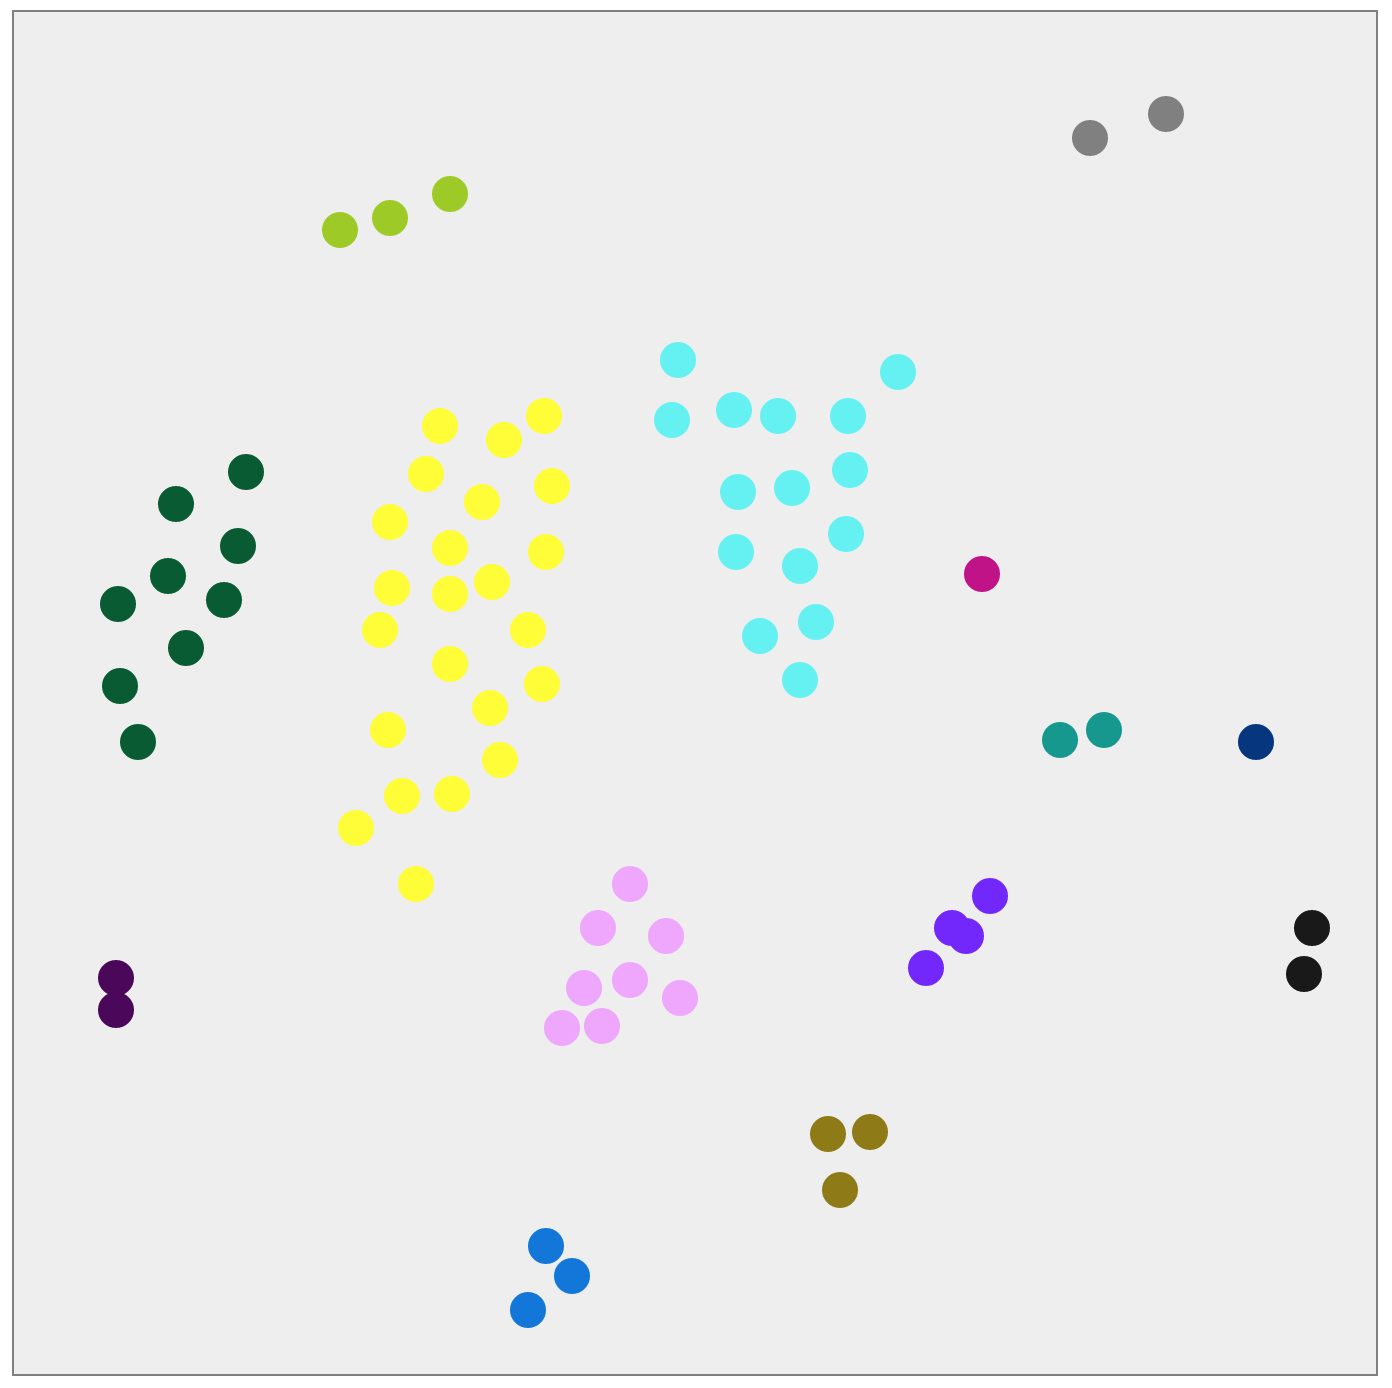
\includegraphics[width = \textwidth]{figures/xp2example.png}
\caption{Spatial and group organization provided by subject 1.
\vl{
Why have you chosen subject 1, who made 14 clusters?
This is an unusually large number, according to the
histogram in Figure 2.
It would be more representative of the population to illustrate this figure
with the data of a subject with the median number of clusters.
It would be good to show the three stages of the human-computer interface:
random initialization,
geometric clustering on screen,
and color clustering.
Besides, the figure is not accessible to readers with
color vision deficiencies at the moment.
The color of the clusters should be reinforced with
geometrical information, \eg{} Voronoi cells.
@data @figure}}
\label{fig:xp2display}
\end{figure}

31 subjects completed the experiment. An example of resulting organization of \ipt is given on Figure \ref{fig:xp2display}. The resulting organization for each subject are available for reader's inspection using the full feature interface provided to the subjects for performing the experiment\footnote{https://mathieulagrange.github.io/paperSpontaneousSimilarity/demo}.

As discussed in the previous section, only the clustering given by the subjects using the color labels is considered to estimate the spontaneous judgments of similarity among \ipt. The spatial organization of the dots representing the \ipt could provide information about the similarity, but this would implicitely force the fact that the timbral similarity space is two dimensional. We therefore now only study the properties of the clusterings performed by the subject prior to converting them into an overall similarity matrix.

Among the 20 colors available, the subjects used on average $10.2 \pm  4.1$ different colors to group \ipt. The distribution of the number of groups can be seen on Figure \ref{fig:xp2nbGroup}. The size of the groups is on average $7.7 \pm   7.2$. The distribution of the size of groups can be seen on Figure \ref{fig:xp2sizeGroup}. The large number of small groups indicates that many subjects considered that a few of the \ipt were very different from all the remaining \ipt.

\begin{figure}
\center
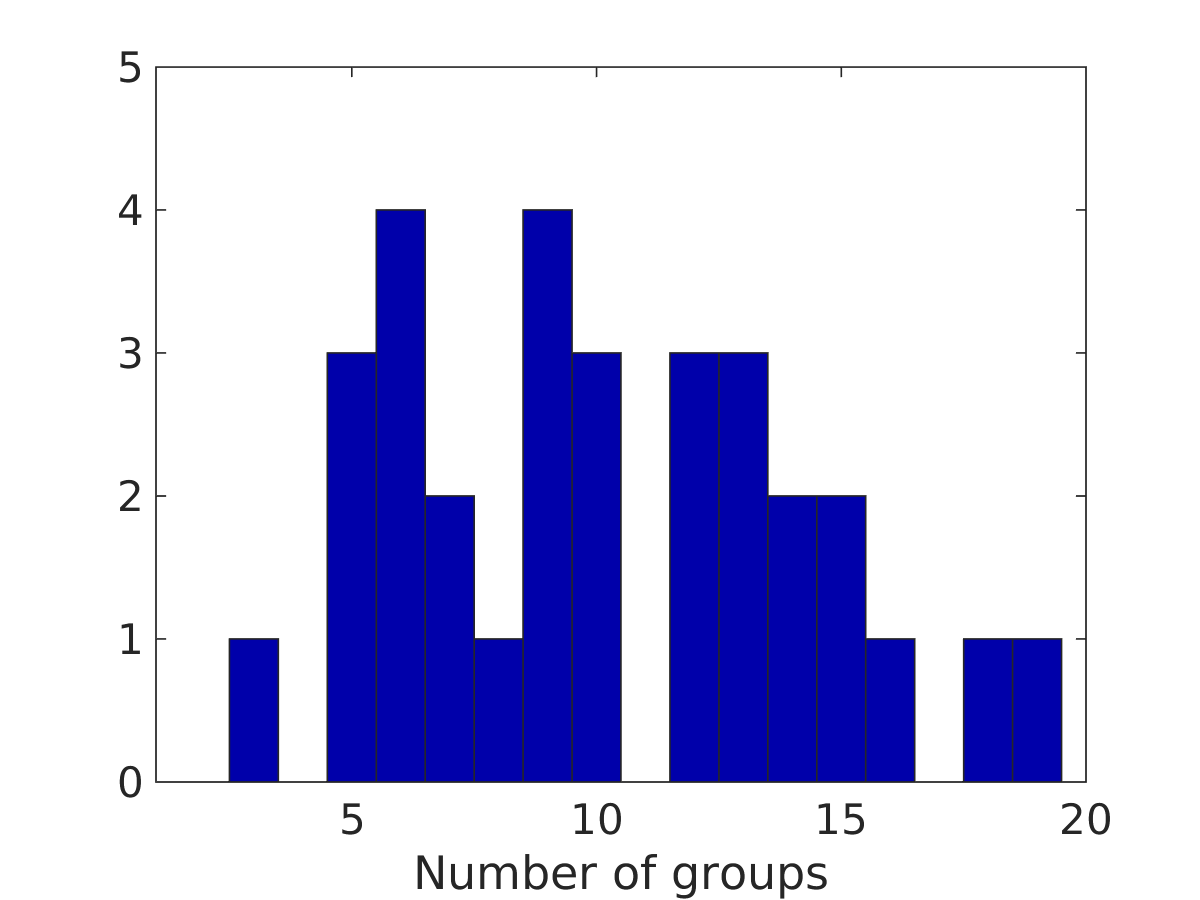
\includegraphics[width = \textwidth]{figures/nbc.png}
\caption{Histogram of the number of groups.
\vl{The width of this figure should be a half page instead of a full page. Pair with next figure. @figure}}
\label{fig:xp2nbGroup}
\end{figure}

\begin{figure}
\center
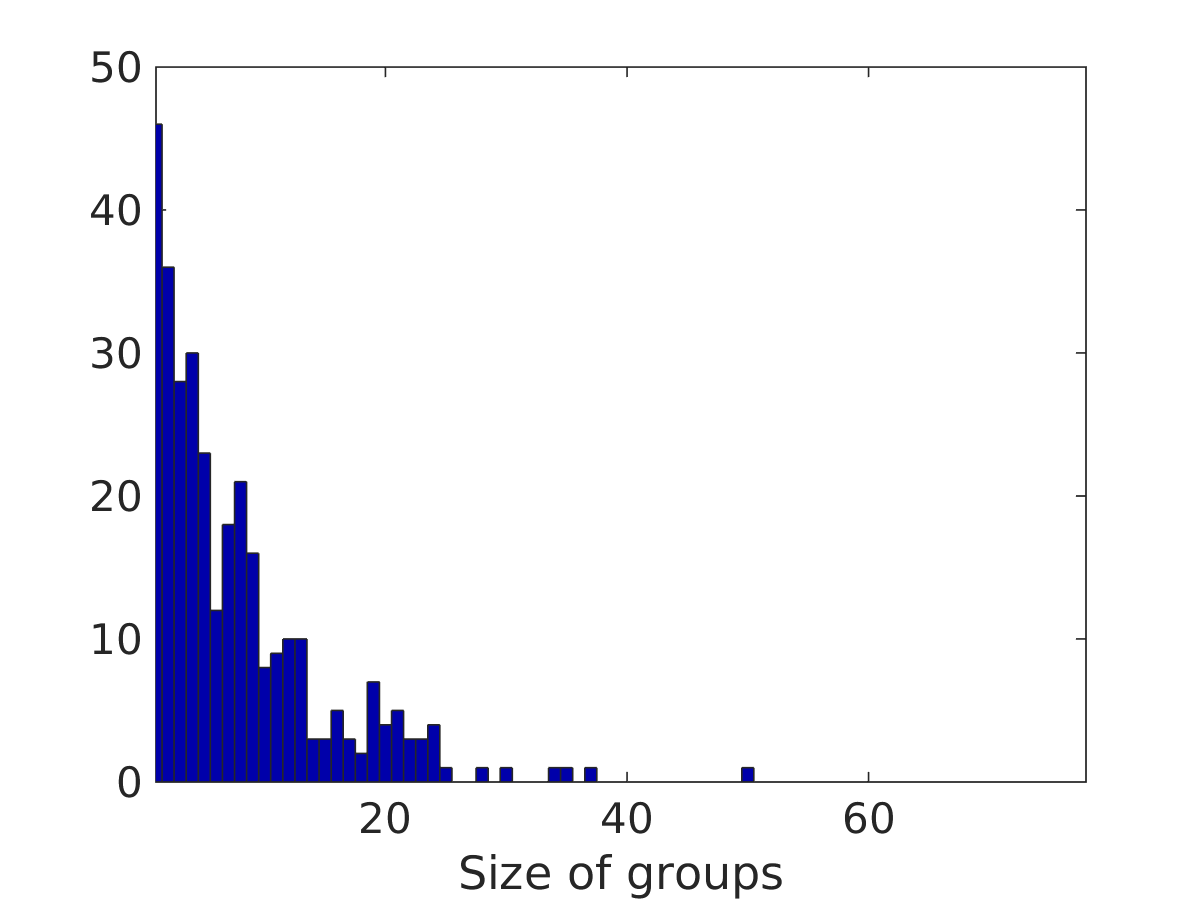
\includegraphics[width = \textwidth]{figures/sbc.png}
\caption{Histogram of the size of groups.
\vl{The width of this figure should be a half page instead of a full page. Pair with previous figure. @figure}}
\label{fig:xp2sizeGroup}
\end{figure}

A clustering can be considered as a binary similarity measure, with $s(a, b) = 1$ if $a$ and $b$ belong to the same group, and $0$ otherwise. By averaging the 31 binary similarity matrix, an overall floating point matrix is obtained that correponds to our measure of the spontaneous perceptual similarity between \ipt.

In order to gather information about the properties of the data, a cluster analysis is next performed using an agglomerative hierarchical clustering \cite{gordon1987review} using the weighted average algorithm for computing distance between clusters. The resulting dendrogram is displayed on Figure \ref{fig:dendrogram}. A partition of $n$ clusters can be constructed from the agglomerative hierarchical cluster tree by finding the smallest height at which a horizontal cut through the tree leaves $n$ clusters.

One question that arises is whether the similarity is influenced primarily by the instrument or by the playing technique. To answer this question, each partition provided by cutting the dendrogram at successive levels is compared to two reference partitions. One reference is the partition of the \ipts when labeled with the instrument used (I) and the other if the partition of the \ipts when labeled with the playing technique used (Pt).

There are many metrics available to compare two partitions by evaluating their degree of correspondance \cite{wagner2007comparing}. The normalized mutual information (NMI) is interesting as it do not require alignement of the groups labels between the two partitions prior correspondance analysis and the two partition are not required to have the same number of groups. It also by design bounded between 0 and 1, 1 meaning perfect match. We consider the normalization proposed in \cite{strehl2002cluster}. Figure \ref{fig:clusters} shows the evolution of the NMI when comparing the partitions provided by the cluster analysis of the dendrogram produced using the human judgment of similarity and respectively the instrument partition ($j/I$) or the playing technique partition ($j/Pt$).

\begin{figure}
\center
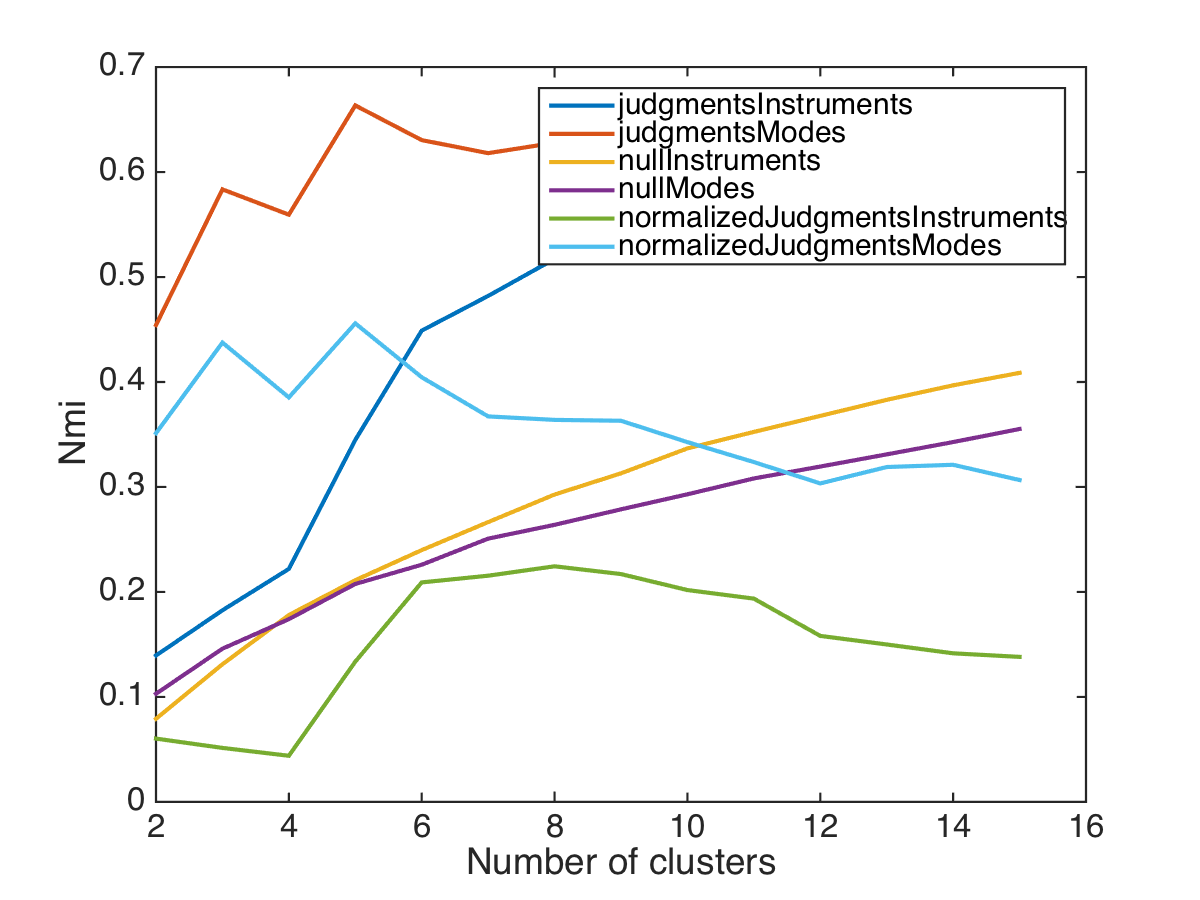
\includegraphics[width = \textwidth]{figures/clusterAnalysis.png}
\caption{Cluster analysis of the similarity judgments. $j/I$ and $j/Pt$ compare the partition obtained using the similarity judgments clustered using a growing number of clusters versus respectively the instrument partition and the playing technique partition. Normalizing null partitions based NMI $nullI$ and $nullPt$ are used to obtain normalized measures: $nj/I$ and $nj/Pt$.
\vl{This line plot is very hard to understand.
The legend box occludes the data on the top-right corner.
It would be preferable to remove this legend box and label lines
by placing text upon them,
so that the plot would be legible to readers with color vision deficiencies.
Besides, the choice of line labels is cryptic, as it relies on abbreviations.
The distinction between I and Pt
can be illustrated by two complementary colors, \eg{} blue versus orange.
The distinction between j, nj, and null
can be illustrated by three distinct markers
(empty circle, filled triangle, asterisk),
associated with
three distinct line styles (solid, dashed, dotted).
The NMI abbreviation should be expanded.
@figure}}
\label{fig:clusters}
\end{figure}

There is a clear gain of NMI when considering the playing technique which means that the subjects primarily used cues corresponding to the playing technique to organize the \ipts. Also, for both curves, a global trend of increase in the $j/x$ partitions with respect to the number of clusters can be observed. This is a well documented fact, which simply put, means that it is easier to match any given partition with more clusters at hand \cite{tibshirani2001estimating}. To compensate for this bias, one can consider the NMI that would be achieved by comparing to the reference partition several random partitions of increasing number of clusters. The resulting averaged NMI for 100 randomly generated partitions is displayed on Figure \ref{fig:clusters}. This so-called null partitions NMI are respectively termed $nullI$ and $nullPt$ depending on the reference used. To normalize $j/I$ and $j/Pt$ in order to reduce the impact of this bias, we simply substract the $null$ NMI:
\begin{eqnarray}
  nj/I &=& j/I - null \\
  nj/Pt &=& j/Pt - null  \\
\end{eqnarray}
This normalization is useful for identifying more easily the number of clusters for which the comparison is most relevant. As can be seen on Figure \ref{fig:clusters}, the number of clusters that leads to the highest NMI is 5 for the playing technique reference and 8 for the instrument reference, leading respectively to an NMI of $0.46$ and $0.21$. For the latter, reducing the number of clusters down to 6 do not decrease the NMI by much, a fact that will be latter discussed in more details. Even by considering the null normalization, the matching level is much higher for the playing technique reference.

The correspondances between those partitions and the reference ones are now studied. For this purpose, Figure \ref{fig:gi} displays two partitions. At the bottom is the partition that corresponds to the instruments labels, whose color code is given by the color bar on the right. The abbreviations used for the instruments are detailed in Section \ref{sec:dataset}. The ordering of \ipts on the horizontal axis is the one given by the cluster analysis, see the dendrogram on Figure \ref{fig:dendrogram}. The partition on top is the result of the clustering with 8 clusters. For visualization purposes, we arbitrarily set colors to clusters of this partition to the color code of the instrument label that is most often encountered in this cluster. If some labels occur equally often, the instrument of the first \ipt of the cluster is chosen. The emerging instrument classes are: Saxophone, Clarinet, Trumpet, Flute and Cello.

Though, even with an optimal number of clusters, we see that the clusters have  a low purity, \ie{} a very diverse set of instruments labels for the \ipt they belong to. Also, some clusters could be merged without stong changes in the overall organization. This probably explains the small changes of NMI when reducing the number of clusters, see Figure \ref{fig:clusters}.

As can be seen on Figure \ref{fig:gm}, the correspondance between the playing technique reference and the resulting partition with 5 clusters is much higher. Most clusters have a high level of purity and for groups emerge : Pizzicato, Slap, Ordinario, and Ponticello.

To conclude this section, the process of gathering data about the perceptual similarity of \ipt is found to be successful as the subjects used their degree of freedom in a consistent manner and no inconsistency in the data has been detected during the analysis process. The main result is that the playing technique is an important factor when modeling the spontaneous judgment of similarity gathered in the second experiment.


\begin{figure}
\center
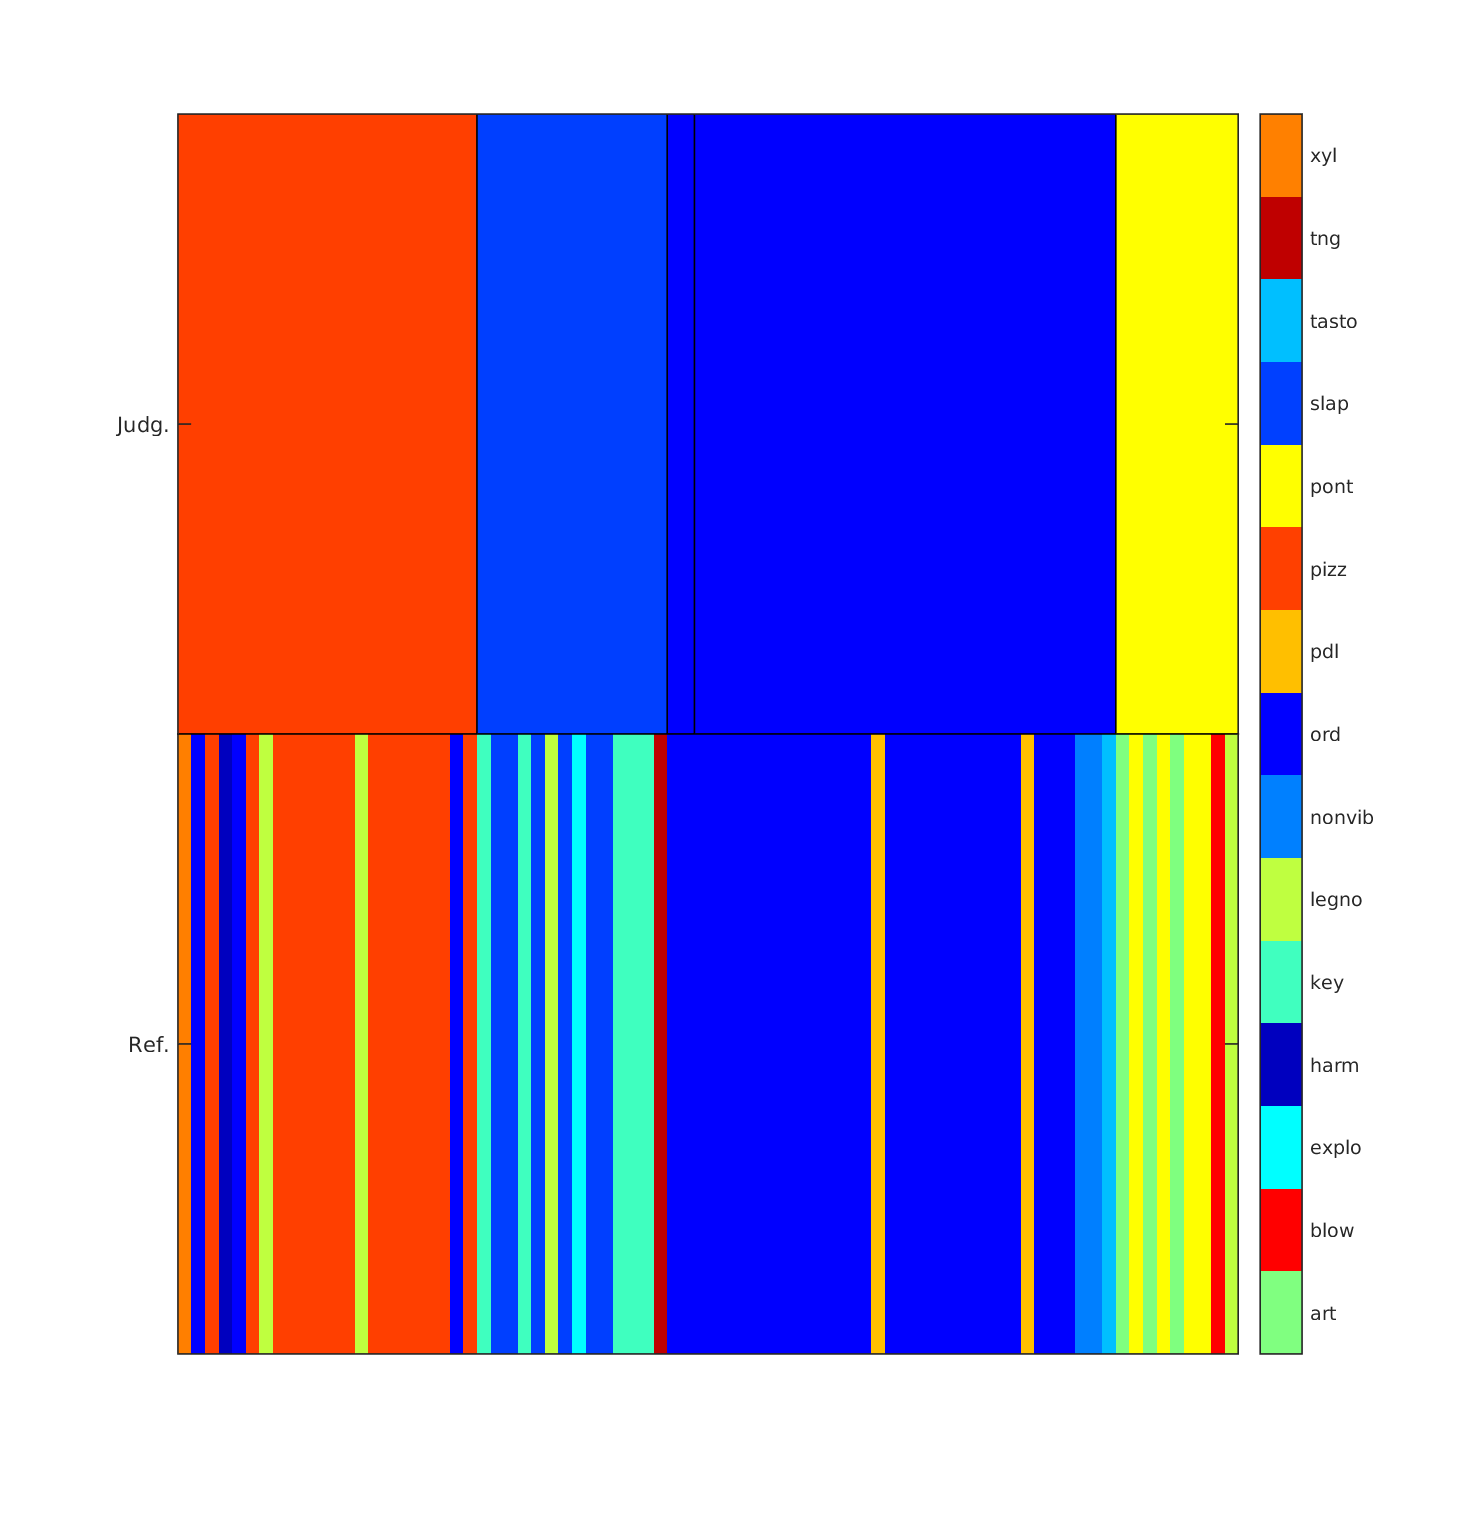
\includegraphics[width = \textwidth]{figures/groupModes.png}
\caption{Clustering \ipts using average perceptual similarity into 5 clusters (top) and playing technique labels (top). The color chosen to display each clusters on top corresponds to the playing technique that is dominant in this cluster, from left to right: 'pizzicato', 'slap', 'key', 'ordinario', 'ordinario', 'ponticello', 'art'.}
\label{fig:gm}
\end{figure}





\begin{figure}
\center
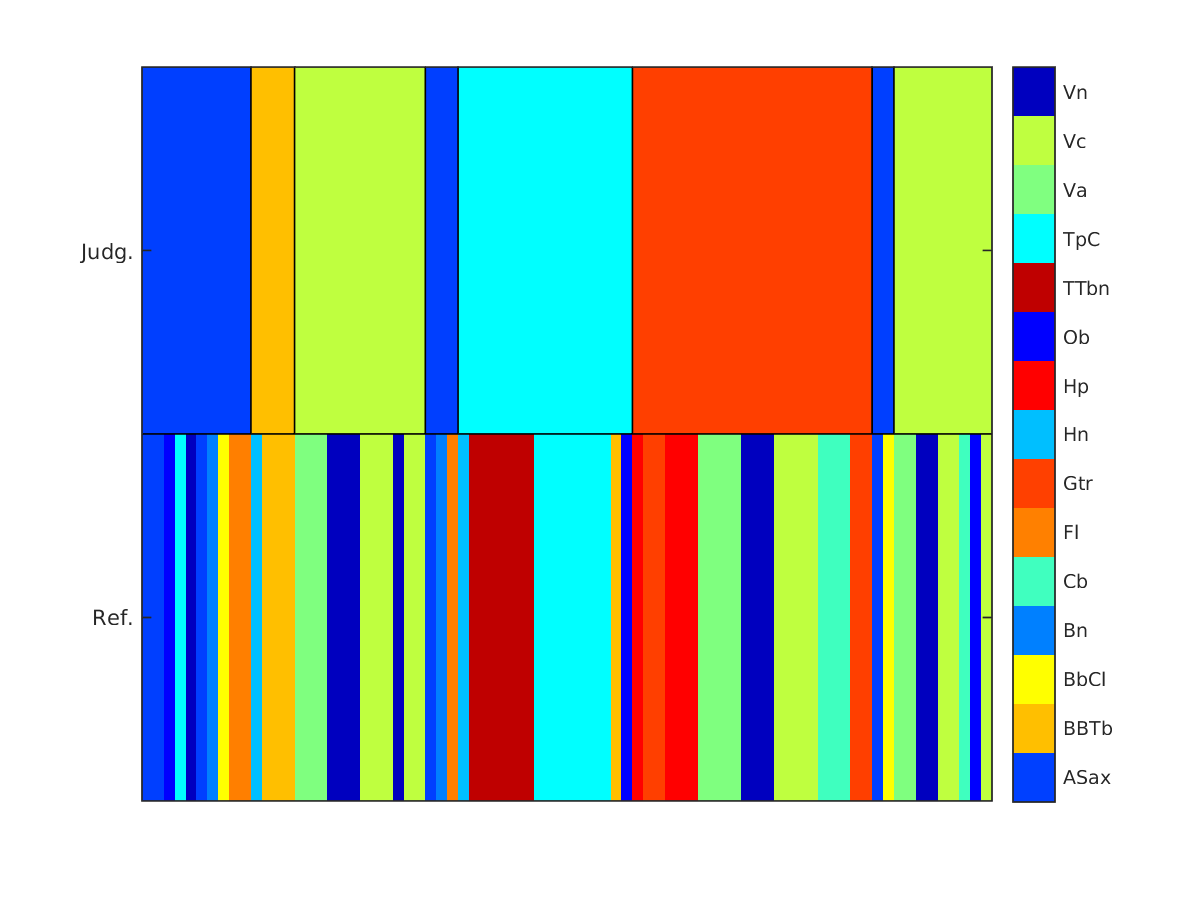
\includegraphics[width = \textwidth]{figures/groupInstruments.png}
\caption{Clustering \ipts using average perceptual similarity into 8 clusters (a) and instrument reference labels (b). The color chosen to display the groups (on top) corresponds  to the instrument that is dominant in this group, from left to right: 'ASax', 'BBTb', 'Vc', 'ASax', 'TpC', 'Gtr', 'ASax', 'Vc'.}
\label{fig:gi}
\end{figure}

\section{Model}\label{sec:model}

Once the perceptual data is gathered and controled, our aim is now to evaluate the ability of the proposed two stages perceptual model brifely described and motivated in the Introduction. The model is composed of two successive processing stages, respectively called the primary and the secondary stage, see Figure \ref{fig:model}. The primary stage is designed to rely on very few meta parameters set arbitrarily by the experimenter to mimic the early stages of the mamalian auditory system. On contrary, the secondary stage rely largely on the data it has to predict and in this respect mimic the high plasticity of the later stages of the mamalian auditory system.

\vl{Naming the two stages "primary" and "secondary" is not very informative.
How about "feature extraction" and "similarity learning"? @writing}

\begin{figure}[t]
\center
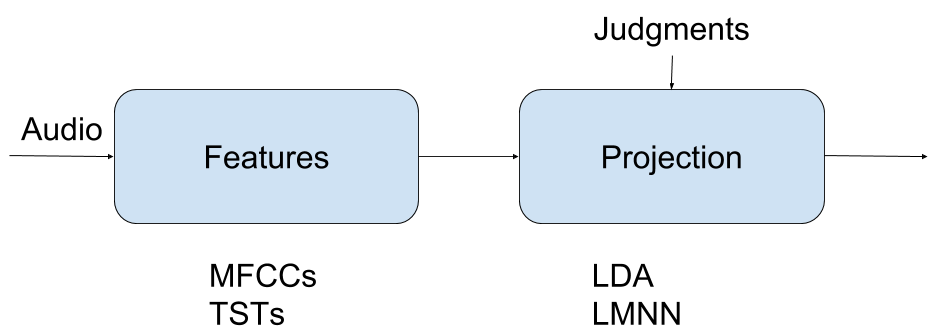
\includegraphics[width = \textwidth]{figures/spontaneousSimilarity.png}
\caption{Computational model composed of two successive processing stages and alternative implementations.}
\label{fig:model}
\end{figure}

\subsection{Primary stage}

In order to model the early stages of the mamalian auditory system, we use the time scattering transform (TST). This transform is obtained by applying a one dimensional
wavelet transform in time to a time-frequency wavelet scalogram \cite{anden2014deep}. It is thus well suited to encode modulations over time of energy distributed over frequency, dimensions that are shown to be perceptually important \cite{dau1997modeling}.

This model is chosen over more data driven alternatives mainly for the sake of simplicity. Deep convolutional networks could have been considered \cite{lee2009unsupervised}, but the learning stage inherent in this kind of methods did not seem relevant for this study. On contrary, the scattering transform can be conveniently parametrized to match the perceptual capabilities of the auditory system as those parameters are not expected to change significantly among subjects. Also, more complex versions of the scattering like the joint time-frequency scattering \cite{anden2015joint} and the spiral scattering \cite{lostanlen2016wavelet} are not considered in order to achieve a projection of reasonable dimensionality and for lack of evidence that those dimensions are mandatory to model the primary stage of the auditory system.

\subsection{Secondary stage}

The secondary stage involves a learning based process block that will weight and linearly combine the features outputed by the primary stage.

Indeed, if the properties of the first processing stages of the human auditory system can reasonably be considered as similar for every subjects despite potential hearing losses for some, the later ones is expected to vary more drastically due to their respective education, tastes and experiences with stimuli similar to the \ipt that are considered in this study. We therefore consider a supervised setting in order to optimize the feature space provided by the scattering transform. To do so, we will consider as our reference the clusterings provided by the subjects of experiment 2. Therefore, the goal of the secondary stage is to provide a metric space that closely match the one resulting from the data gathered by experiment 2.

To do so, one can first consider the linear discriminant analysis (LDA) \cite{duda2000pattern} to project the data into a representational space of $C-1$ dimensions with $C$ being the number of clusters of the reference. In our case study, the reference is the partition of \ipts provided by a subject during experiment 2. The projection computed using this method is such that the ratio of the between-class distance to the within-class distance is maximized, thus achieving maximum discrimination between elements of different clusters.

Another solution is to compute a projection matrix that maximizes the fact that neighbors in the representational space belong to the same cluster in the reference clustering while items from different clusters are separated by a large margin. To do so, the large margin nearest neighbor (LMNN) metric learning algorithm \cite{weinberger2006distance, weinberger2009distance} is considered. One advantage of the latter is that the resulting representational space is of the same dimensionality as the input one whereas the LDA output dimentionality is contrained by the number of classes in the reference clustering.

An important issue is that those methods are designed for considering only one reference clustering. It is thus suited to model the perceptual space of one subject but not many. However, in our case, we would like to model a perceptual space that is shared among subjects. One approach is to find a consensus clustering that maximally represent the 31 reference clusterings. To implement this solution, the chosen consensus clustering is taken from 3 solutions issued from 3 different algorithmic approaches introduced in \cite{strehl2002cluster}. This consensus clusterings is chosen among the 3 solutions as the one that has the best averaged NMI when compared to the 31 reference clusterings.

Another approach is to combine the projection matrices issued from the processing of the projection algorithm over the 31 reference clusterings. As the number of classes can vary between reference clusterings, the kind of combination is not feasible using the LDA method. On contrary, the LMNN method aloways outputs a projection matrix with equal dimensions. Those projection matrices being of the same dimensionality they can safely be averaged to estimate an consensus projection.

\section{Validation}\label{sec:validation}

As it will be discussed in the next Section, the main application scenario that is considered in this paper is the recommandation of sounds based on examplar. This involves the definition of a similarity measure that behave similarly to the human perception. In this paper, the reference used for assessing closseness to human perception is the perceptual data gathered in experiment 2.

Our problem is thus casted into a ranking problem, where from several candidates, the algorithm is asked to provide a ranking list of those candidates, sorted by similarity.

\subsection{Data}

As explained in the first section, gathering perceptual similarity data is plagued is plagued with a size problem. Thus, the perceptual data considers 78 \ipts each represented by one sound recording, most often of C4 pitch and nuance mezzo forte. In order to provide enough data for the numerical analysis described in this section, we complement the data gathered during the second experiment as follows: for each \ipt, instead of one sound examplar we consider the whole range of nuance and pitch that is available. This leads to a dataset of 9346 sound recordings. It is thus assumed that the perceptual similarity is invariant with respect to pitch and nuance which is not necessarily true, but is taken in this paper as a reasonable assumption.
\vl{It's too bad that this "reasonable" assumption is not challenged against the data. In music psychology, the "bandwidth for timbre invariance" is of the order of one octave (Handel and Erickson, Music Perception, 2001) or less (Steele and Williams, Music Perception, 2006).
One way to do it without collecting new similarity judgments would be to break down the precision by pitch of query.
Presumably we have an inverted U shape with a peak near C4.
@research @computation @figure @biblio}

\subsection{Metric}

The performance of the different methods are evaluated in a ranking setting. The precision at rank $k$ is thus considered, with $k=5$. For one sound recording taken as the query, the $k$ nearest sound recordings are retrieved from the remaining items of the database. The precision is the number of neighbors that have the same label as the query in the clustering we consider as reference divided by $k$. For example, if a sound is played by a Violin, and among the 5 nearest neighbors of this query sound, 2 are played by a Violin, the precision is $0.4$. This process is repeated for each sound recordings taken as query, and the performance is averaged over all the queries.

When considering several clusterings as reference, the precision is averaged per clusterings. In our case, the precision is thus computed for the 31 reference clusterings and averaged.

\subsection{Methods}

To evaluate the performance of the proposed approach, several baselines are considered for comparison purposes. For the first stage, the well known Mel-Frequency Cepstral Coefficients (MFCC)s are considered \cite{rabiner1993fundamentals}. The MFCCs are computed from audio frame of 25ms to 1 second, the number of mel bands is 40 and all the discrete cosine transform coefficients are kept. The resulting features have thus a dimensionality of 40. The MFCCs are then standardized by removing the mean and dividing by the standard deviation computed over the whole dataset.

The time scattering transform is computed over a range frame sizes, from 25 ms to 1 second. The Q factor is set to 8 in order to obtain a frequency decomposition that is equivalent to the mel scale \vl{The mel scale has a varying quality factor, so I don't see how this can be right}. As the frame size increase, the dimensionality increases. Unless otherwise stated, the frame size is one second. The resulting scattering features are then logarithmically compressed and normalized using the median computed over the whole dataset.

The LDA method do not requires any setting of parameters and the LMNN method is set to optimize for a neigbors size of 5.

\subsection{Results}

In order to validate the proposed model, experiments are performed using the above described methods. 3 experimental factors with 2 to 3 modalities are considered:
\begin{itemize}
  \item type of features: MFCCs or TST
  \item type of projection: LDA, LMNN
  \item type of reference for the optimization of the projection if any: consensus (single consensus clustering) or multiple (the 31 reference clusterings)
\end{itemize}
The results are shown on Table \ref{tab:res1}. Considering the TST over the MFCCs to implement the primary stage do not improve by much (2 \%) if no secondary stage is used. When the best setting of the secondary stage is considered, the gain is higher (7 \%). this potentially mean that the extra capabilities of description of the TST over the MFCCs need to be targeted to the task at hand in some way in order to gain the full benefits from its use.

In terms of projection method to implement the secondary stage, the LMNN approach is favored over the LDA, probably due to the fact that the dimensionality reduction induced by the low number of classes relatively to the number of dimensions of the input space strongly degrades the description capabilities of the resulting projection. The lower performance of the LDA with respect to no projection is probably partly due to that and the fact that the metric is not computed on the consensus clustering use for computing the LDA.

In this experiment, the consensus approach is favored for TST but not for MFCCs. This approach has the considerable advantage of being more computationaly efficicient as with only one reference to optimize from the LMMN training is much faster. Though, it is very likely that for a larger number of reference clusterings, the multiple LMNN would be useful to better model the diversity of the references.


\begin{table}
  \caption{Precision achieved by the different settings. Numbers in bold face indicate best performance. \vl{Why are the results with TST, LMNN, and "reference" commented? Do they correspond to same rater between training and evaluation? @methodology}}
  \label{tab:res1}
  \begin{center}
\begin{tabular}{lllc}
features & projection & reference & precision (\%) \\
  \hline
  MFCCs & - & - &   85.07 $\pm$ 6.19 \\
  MFCCs & LDA &  consensus  &   81.50 $\pm$ 7.65 \\
MFCCs & LMNN & multiple & 86.31 $\pm$ 5.91 \\
MFCCs & LMNN & consensus &   86.22 $\pm$ 5.92 \\
% MFCCs & LMNN & reference &   86.18 $\pm$ 6.05 \\
TST & - & - &   87.01 $\pm$ 5.81 \\
TST & LDA & consensus &   80.95 $\pm$ 10.37 \\
TST & LMNN  & multiple  &   93.31 $\pm$ 3.92 \\
TST & LMNN & consensus &   \textbf{94.80 $\pm$ 3.26} \\
% TST & LMNN & reference &   98.09 $\pm$ 1.28 \\
\end{tabular}
\end{center}
\end{table}

We now investigate the influence of the frame size, as it is likely that the more observation time is available, the better the description will be as several playing techniques involve strong modulations over long periods of time. We therefore consider a frame size for the 2 sets of features ranging from 25 ms. to 1s. The evolution of the precision with respect to the frame size is shown on Figure \ref{fig:frame}. Even by enlarging the frame size, the performance of the MFCCs do not increase due to the lack of modulation's modeling. On contrary, the TST is able to use the larger frame size to achieve better precision.

\begin{figure}
\center
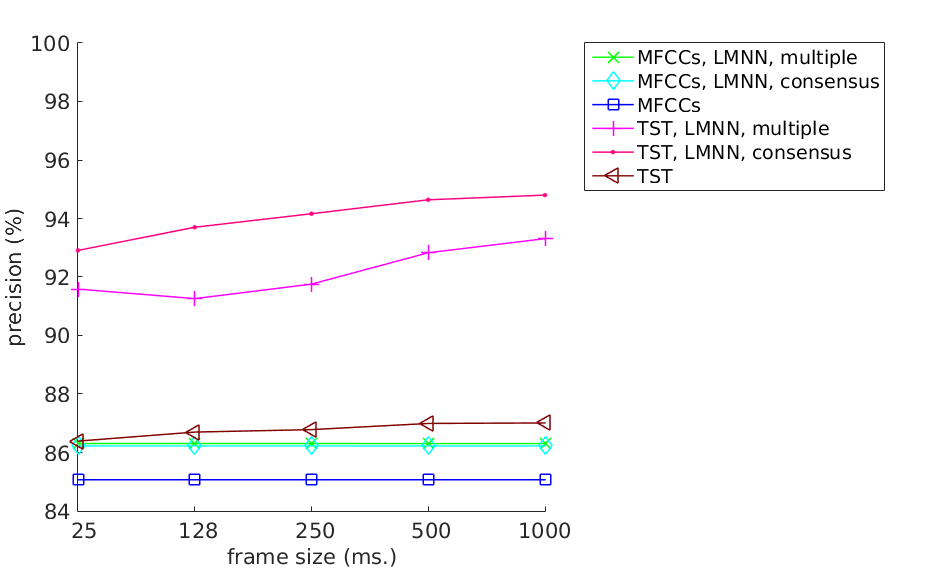
\includegraphics[width = \textwidth]{figures/frame.png}
\caption{Spatial and group organization provided by subject 1.}
\label{fig:frame}
\end{figure}

An interesting phenomenon appears, the gain of performance due to the larger frame size better improves for the TST if the secondary stage is considered. Again, it seems that enriching the description is most useful if the description is optimized with a purpose.

We investigated the capabilities of the proposed system to model a perceptual space averaged over several subjects. For application purposes that will be discussed in the next Section, it can be useful to consider the reference clustering of only one user and see if the system perform well with this kind of reference. To do so, the evaluation protocol is slightly modified. First the secondary stage is optimized for the 31 reference clusterings independantly and for each resulting projection the precision is computed. The 31 precision measures are then averaged and shown in Table \ref{tab:res2}. The excellent results of the TST optimized using LMNN demonstrates the usefullness of the proposed approach to model complex similarity space such as the percpetual ones gathered in Experiment 2.


\begin{table}
  \caption{Precision achieved when considered subject based reference clusterings. Numbers in bold face indicate best performance.}
  \label{tab:res2}
  \begin{center}
\begin{tabular}{llc}
features & projection & precision (\%) \\
  \hline
MFCCs & LMNN & 86.18 $\pm$ 6.05 \\
TST & LMNN & 98.09 $\pm$ 1.28 \\
\end{tabular}
\end{center}
\end{table}


For the sake of reproducibility, the code of the proposed method and the experimental protocol is available\footnote{https://github.com/mathieulagrange/paperSpontaneousSimilarity}. For convenience, the features (scattering and mfccs) are also provided, but the software can be used to process audio data.

\section{Discussion}\label{sec:discussion}

Thanks to the digitization capabilities available, gathering large amount of audio recordings of \ipt is achievable and several databases are now available on the market. Browsing of such databases can be achieved by keyword based search. It requires that 1) the database is fully annotated with a precise ontology of instruments and playing techniques, 2) that the user has a precise understanding of this ontology, and 3) that the user a precise idea of the kind of timbre he is looking to find the \ipt he is searching for.

An interesting alternative type of search is the similarity content based search. Being solely based on sound, this kind of search can be used when querying by example. The user provides an example of the target sound to find \ipt that match the timbre description of the query, be it an onomatepea, a tone from another instrument or any kind of sound.

The computational model proposed in this paper is well suited for this kind of search, as it can model complex perceptual timbre spaces and can scale to large databases. Once the features and the projection matrix are computed, the similarity computation is quite effective and can be further enhanced by considering fast similarity search scheme such as locally sensitive least square hashing \cite{pauleve2010locality}. The secondary stage being learnt, it can easily adapt to user tastes and usage history by reweighting the features for improved search relevance.

\section{Conclusion}

The modeling of the spontaneous perceptual similarity have been studied. Experimental data have been collected using two perceptual tests whose outomes have been analysed to produce reference data of spontaneous perceptual judgments. This data is then modeled computationaly using a two step model.

The first step considers the use of the time scattering transform that is well suited for modeling acoustic signals whose spectrum is modulated over time. This transform is considered to induce a perceptual feature space that is transformed by the second step that consist in a learning based projection.

Computational experiments showed an interesting phenomenon that high dimensional features spaces such as the one achieved using the TST are most useful if another computation step is considered, if this second step is able to incorporate some sort of prior knowledge regarding the task at hand in order to refine the resulting representation. It would be interesting to verify if this phenomenon can be observed for other types of targeted tasks, using larger datasets and with a higher level of control regarding the learning procedure to study the impact of potential overfiting or learning biases of this king of techniques.


%%%%%%%%%%%%%%%%%%%%%%%%%%%%%%%%%%%%%%%%%%%%%%%%%%%%%%%%%%%%%%%%%%%%%%%%%%%%%%%%
%%%%%%%%%%%%%%%%%%%%%%%%%%%%%%%%% ACKNOWLEDGMENTS %%%%%%%%%%%%%%%%%%%%%%%%%%%%%%
\section*{Acknowlegments}

The authors would like to thank
PSL for funding this research,
CNSMDP for fruitful collaboration,
and Ircam for providing access to the SOL database.


%%%%%%%%%%%%%%%%%%%%%%%%%%%%%%%%%%%%%%%%%%%%%%%%%%%%%%%%%%%%%%%%%%%%%%%%%%%%%%%%
%%%%%%%%%%%%%%%%%%%%%%%%%%%%%%%%% BIBLIOGRAPHY %%%%%%%%%%%%%%%%%%%%%%%%%%%%%%%%%

\bibliographystyle{alpha}
\bibliography{bib}

\section{Dataset} \label{sec:dataset}

The dataset considered in this paper as been recorded at Ircam and is composed of audio recording of 16 different musical instruments played with different playing techniques, which leads to 143 different couple of instrument / playing technique. For each couple, the pitch and intonation is varied leading to 25444 audio samples.

The recorded instruments belongs to the wind and string classes. For winds, the instruments considered in the second experiment are: accordion (Acc), saxophone alto (ASax), tuba (Tb), bassoon (Bn), clarinet Bb (BbCl), flute (Fl), horn (Hn), oboe (Ob), trombone tenor (TTbn), and trumpet C (TpC). For the string class, the instruments are: guitar (Gtr), harp (Hp), viola (Va), violin (Vn), violoncello (Vc), and contrabass (Cb).

Some instruments can be complemented with sordina (S), wha (W). The addition of this kind of device modifying the shape of the instrument, a saxophone alto and saxophone alto with sordina are considered as different instruments.

Those instruments are recorded for different nuance and pitch if the latter is relevant, but more importantly, several playing technique are considered. For  the second experiment described in this paper, the playing techniques considered are: artificial harmonic (art), blow (blow), exploding slap  (explo), harmonic (harm), key-click (key), col legno   (legno), non vibrato (nonvib), ordinario (ord), pedal tone (pdl), pizzicato (pizz), ponticello (pont), slap (slap), (tasto), tongue-ram (tng), and xylophonic (xyl).

\vl{This section is not precise enough in terms of intensity ranges and pitch ranges.
The abbreviations can be removed. @data @writing}

\vl{A bubble plot of number of notes per instrument (x axis) and playing technique
(y axis) would be extremely useful. @data @figure}

\section{Dendrogram}

\begin{figure}
\center
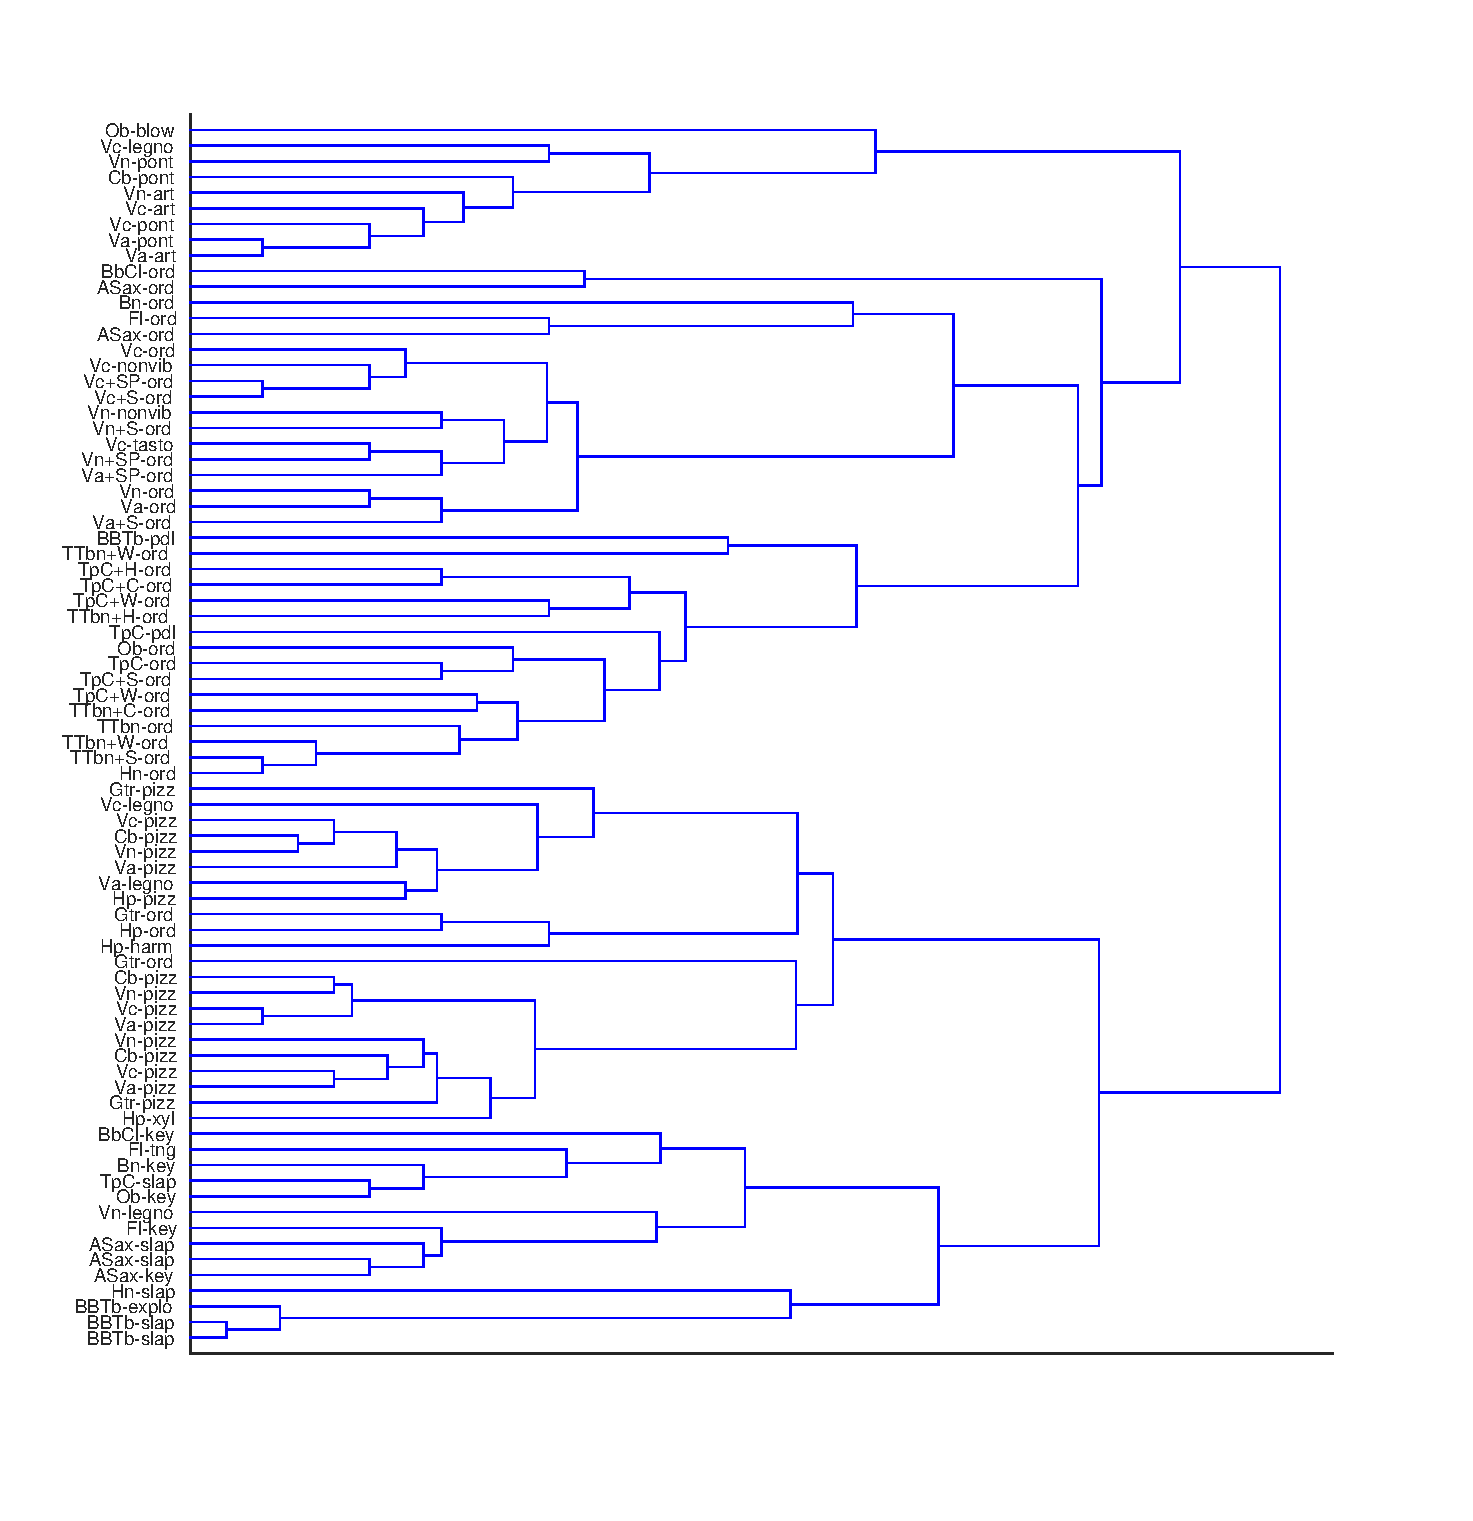
\includegraphics[width = \textwidth]{figures/dendrogram.pdf}
\caption{Dendrogram obtained after processing the similarity judgment matrix using the agglomerative clustering algorithm.}
\label{fig:dendrogram}
\end{figure}

\vl{This dendrogram is very hard to read. Abbreviations must be replaced by the full names of every instrument and playing tecniques.
Another way to visualize it would be a two-dimensional embedding, such as t-SNE or Isomap (I'm biased towards Isomap). @figure
}

\end{document}
